\documentclass[11pt,letter]{exam}
\topmargin -0.15in \textheight 8.5in \textwidth 6.5in \oddsidemargin
0in \evensidemargin 0in
\usepackage{graphicx}
\usepackage{amsmath, amssymb}
\newcommand{\ben}{\begin{enumerate}}
\newcommand{\een}{\end{enumerate}}
\usepackage{amsfonts}

\usepackage{color}
\usepackage{graphicx}
\usepackage[latin1]{inputenc}
\usepackage{tikz}
\usetikzlibrary{trees}
\usepackage{verbatim}



\begin{document}

% Set the overall layout of the tree
\tikzstyle{level 1}=[level distance=3.5cm, sibling distance=2.5cm]
\tikzstyle{level 2}=[level distance=3.5cm, sibling distance=1.5cm]

% Define styles for bags and leafs
\tikzstyle{bag} = [text width=4em, text centered]
\tikzstyle{end} = [circle, minimum width=3pt,fill, inner sep=0pt]

\CorrectChoiceEmphasis{\color{red}\bfseries}
\bracketedpoints
\pointpoints{pt}{pts}
\setlength\answerskip{0.05ex}

\begin{center}
{\Large {\bf CMSE 381  Final Exam} }
\end{center}
\vspace{1cm}

April 27, 2020 \hfill Time allowed: 120 minutes \vspace{1 cm}

{\bf Name: \underline {\hspace{2in}}} \hspace{1cm}

\vspace*{0.7in}

{\bf Pledge}: {\it I have neither given nor received any unauthorized aid during this exam.}
\vspace*{1.25cm}\\
Signature \rule{5cm}{.5mm}\vspace*{0.7in}

{\bf Instructions:}\\
\vspace*{.1in}
\\
For all the questions, show all your work in the space provided. You will NOT receive credit if you do not justify your answers. \\
\vspace*{.1in}\\
This is a closed book and closed notes examination.
\vspace*{.1in}\\
Please budget you time so that you have sufficient time to do all the  questions.


\mbox{}

\makebox[5.5in]{\hrulefill}\\



\vspace*{0.2in}
 {\bf Good luck!}
\newpage

%%%%%%%%Multiple Choice (30 Questions: 2 points a piece)%%%%%%%%%%%%%%

%%%%%%%%Multiple Choice (30 Questions: 2 points a piece)%%%%%%%%%%%%%%
\begin{questions}

\item (10 pts) Suppose that we wish to invest a fixed sum of money in two financial assets that yield returns of $X$ and $Y$ ,
 respectively, where $X$ and $Y$ are  random quantities. We will invest a fraction $\alpha$ of our money in $X$, and will invest the remaining
  $1 - \alpha$ in $Y$. Since there is variability associated with the returns on these two assets, we wish to choose $\alpha$ to minimize the total
 variance of our investment.  Namely, we want to minimize  $\text{Var}(\alpha X + (1 - \alpha)Y )$.
  One can show that the value that minimizes the risk is given by
  \[
  \alpha = \frac{\sigma^2_Y - \sigma_{XY}}{\sigma^2_{X} + \sigma_Y^2 - 2 \sigma_{XY}},
  \]
where $\sigma^2_X = \text{Var}(X)$, $\sigma^2_Y = \text{Var}(Y)$, and $\sigma^2_{XY} = \text{CoV}(X, Y)$. We collect 500 pairs of $X$ and $Y$ as $\{(x_1, y_1), \ldots, (x_{500}, y_{500}) \}$ from  which we can use to estimate $\alpha$. If we want to obtain a 95 \% confidence interval for $\alpha$, what method will you use (CV, LOOCV, Validation set, Boostrap, Random Forest, Boosting, or etc)? Briefly describe the procedure. (please write your answe on a white paper)

\newpage
\question[10] We have a dataset $\{ (x_1, y_1), \ldots, (x_{500}, y_{500}) \} $ with sample size 500, where $x_i \in \mathbb{R}^{100}$ and $y \in \mathbb{R}$. 
 We want to performed a forward step-wise selection on this data set.  Forward stepwise selection begins with a model containing no predictors, and then adds predictors
to the model, one-at-a-time, until all of the predictors are in the model. In particular, at each step the variable that gives the greatest additional improvement to the fit is added to the model.
Hence, we obtained $p + 1$ models $(\mathcal{M}_0, \ldots, \mathcal{M}_p)$ which contain $0, 1, 2, . . . , p$ predictors respectively. Finally, we will select a single best model from among $\mathcal{M}_0, \ldots, \mathcal{M}_p$ using either AIC or BIC. If we want to have a sparse model (the number of predictors is small), which one should we use?  Justify your answer.  (Please write your answer on a white paper)
\newpage

\item Suppose we estimate the regression coefficients in a linear regression model by minimizing 
\[
	\sum_{i = 1}^n \left( y_i - \beta_0 - \beta_1 x_{i1} - \beta_2 x_{i2} \right)^2 \ \ \text{subject to } |\beta_1| + |\beta_2| \leq s,   
\]
for a particular value of $s$. 
\begin{itemize}
	\item[a.] (10 pts) Let $\beta_1$ be the $x-$axis and $\beta_2$ be the $y-$axis. Draw the area of $(\beta_1, \beta_2)$ such that $|\beta_1| + |\beta_2| \leq s$ and illustrate why this procedure will lead to a sparse solution when $s$ is small. 
	\item[b.] (5 pts) As we increase $s$ from 0, how will the training RSS change?  
\end{itemize}

\newpage

\item Suppose that a curve $\hat{g}$ is computed to smoothly fit a set of $n$ points
using the following formula:
\[
	\hat{g} = \text{argmin}_g \left( \sum_{i= 1}^n (y_i - g(x_i))^2 + \lambda \int [g^{(m)}(x) ]^2 dx  \right), 
\]

where $g^{(m)}$ represents the $m$th derivative of $g$.
\begin{itemize}
	\item[a.] (10 pts) If $m = 2$ and we increase the value of $\lambda$, how will the function $\hat{g}$ change (smoother or  rougher)?  and how will it affect the bias-variance trade-off?
	\item[b.] (5 pts)  If $\lambda = \infty, m = 3$, what will be the form of $\hat{g}$? (linear, quadratic, cubic, ridge, LASSO or spline). Justify your answer. 
(Please write your answer on a white paper)
\end{itemize}

\newpage
\item (10 pts) Sketch the tree corresponding to the partition of the predictor space illustrated in the left-hand panel of the following figure. The numbers inside the boxes indicate the mean of $Y$ within each region.\\
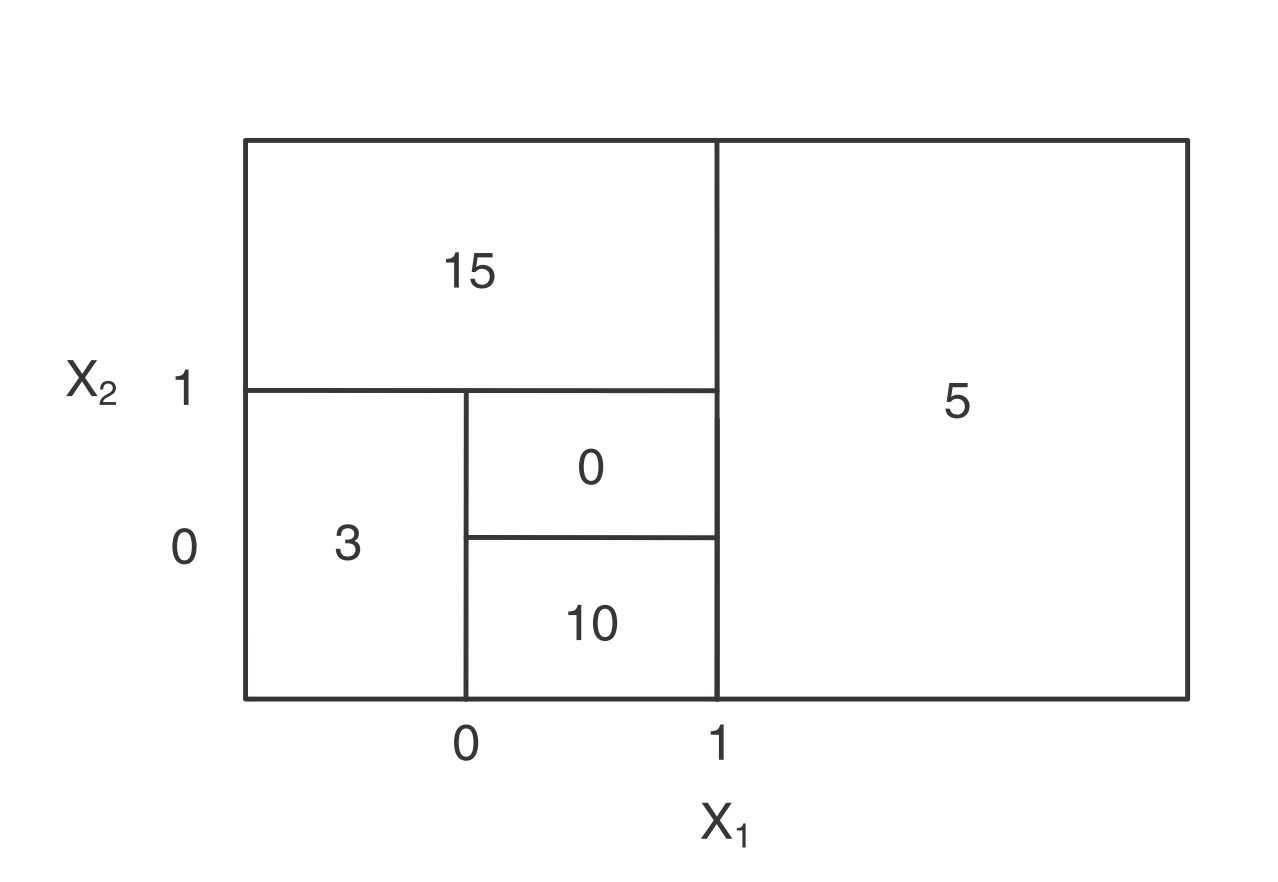
\includegraphics[scale=1]{fig1.png}
\vspace{2 in}

\question[10] How will you estimate the test error of a Random Forest model? Briefly describe the procedure. 
\newpage


\question To build a support vector classifier for non-separable data, we will solve the following optimization problem
\begin{align*}
&\text{maximize}_{\beta_0, \ldots, \beta_p, \xi_1, \ldots, \xi_n, M} M \\
&\text{subject to} \sum_{j= 1}^p \beta_j^2 = 1,  \\
& y_i(\beta_0 + \beta_1 x_{i1} + \cdots + \beta_p x_{ip}) \geq M(1 -\xi_i),
\xi_i \geq 0, \sum_{i =1}^n \xi_i \leq C, 
\end{align*}
where $C$ is a nonnegative tuning parameter. 
	\begin{itemize}
	\item[a.] (10 pts) The slack variable $\xi_i$ tells us where the $i$th observation is located, relative to the hyperplane and relative to the margin. Describe the location of the $i$th observation when $\xi_i = 0$, $ 1 > \xi_i >0$, and $\xi_i \geq 1$.
	\item[b.] (5 pts) After solving the optimization problem, how will you use the SVM model to classify a new observation $x^*$?
	\item[b.] (5 pts) Using the training data $\{(x_1, y_1), \ldots, (x_n, y_n)  \}$, how will you generate the ROC curve for this SVM model?
	\end{itemize}
\newpage

\question[10] We collect 1965 noisy images with pixels $20\times 28$ for each image. Some sample images are shown in the following figure. If we want to denoise those images, what method would you use? Describe your procedure step-by-step.\\
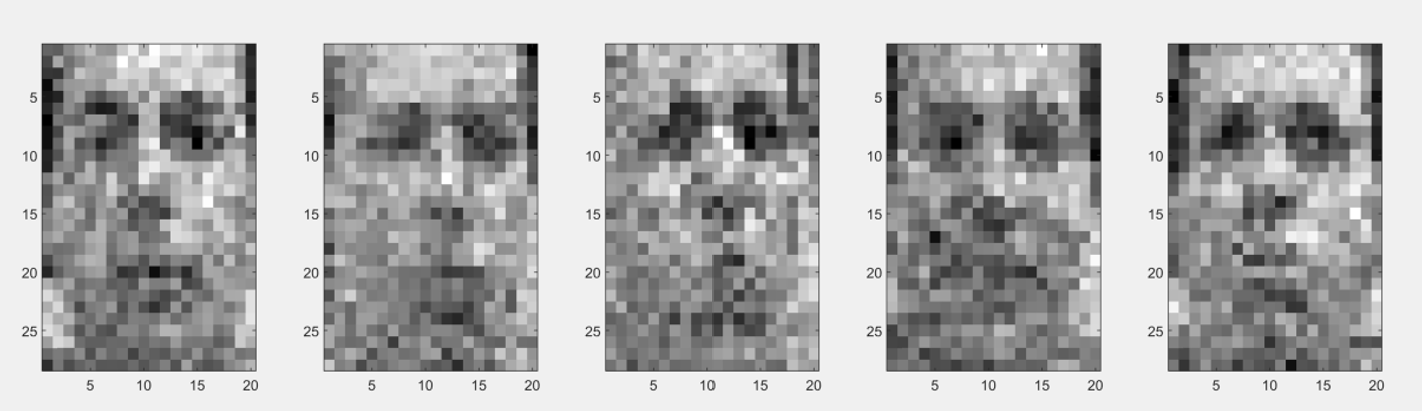
\includegraphics[scale=1]{fig2.png}

\vspace{3 in}
\item (Extra 10 pts) For a classification problem with $K = 2$ ($Y \in \{0, 1\}$), we know the oracle classifier is 
	\[
	C(x) = j, \ \ \text{if $\text{Pr}(Y = j | X = x) = $ max $\{ \text{Pr}(Y = 0 | X = x), \text{Pr}(Y = 1 | X = x) \}$},
	\]
	which is based on the loss with equal weight for Type I and II error. If we know Type I error will cost \$30 while Type II error will cost \$10. Derive the best classifier which minimizes this cost. Namely, given a new $x^*$, how should we predict the label $Y$? (Please write your answer on a white paper)



\end{questions}


\end{document} } 